\documentclass[12pt,a4paper]{article}

% Margins.
\setlength{\oddsidemargin}{0in}
\setlength{\evensidemargin}{0in}
\setlength{\headheight}{12pt}
\setlength{\headsep}{0pt}
\setlength{\topmargin}{-60pt}
\setlength{\textwidth}{6.5in}
\setlength{\textheight}{10.75in}

\usepackage{amsmath}
\usepackage{float}
\usepackage{graphicx}
\usepackage[hyphens]{url}
\usepackage{hyperref}	% Clickable links to figures, references and urls.
\usepackage{datetime}
\usepackage{longtable}

% Drawing.
\usepackage{pgf}
\usepackage{tikz}

% Listings for formatting code.
\usepackage{listings}
\usepackage{textcomp}
% General options.
\lstset{breaklines=true, basicstyle=\small\ttfamily, tabsize=4, numbers=left, stepnumber=1, frame=single, showstringspaces=false, upquote=true}
% C++ specific high-lighting. Comments are 50/50 shades of green/black and strings coloured with 60/40 red/black mixture.
\lstset{language=[ISO]C++, commentstyle=\color{green!50!black}, keywordstyle=\color{blue}, stringstyle=\color{red!60!black}}

%opening
\title{Introduction to Computing\\Lab 03\\Integer Representation and Memory Map}
\author{Moomal Bukhari\and Attique Dawood}
\date{March 03, 2015\\[0.2cm] Last Modified: \today, \currenttime}
\begin{document}
\maketitle
This lab is about representation of integers. Students will use the debugger to learn exactly how the variables are represented and stored as binary numbers in computer memory\footnotemark.

\footnotetext[1]{It is assumed that students are familiar with Visual Studio and basic debugging functions like starting debugger, single-stepping, adding watches and breakpoints. You can refresh these concepts by referring to the \emph{Debugging} section in \emph{Creating a New Project in Visual Studio}}

\section{Storing Signed/Unsigned Integers}
It is imperative that you feel comfortable with binary and hexadecimal conversion. Following sections cover a few basic concepts.

\subsection{Binary and Hexadecimal Conversion}
Conversion between binary and hexadecimal notation is straightforward. To convert a binary number, divide it into groups of four bits starting from least significant bit. Add additional zeros to the most significant bit to make the total number of bits a multiple of four. Hexadecimal (or hex) notation is convenient because it saves space. Notice, any number starting with \verb|0x| is a hex value.

\begin{table}[H]
\centering
\label{4-bit-bin-hex-table}
	\begin{tabular}{l c l}
	\hline \hline \\ [-2ex]
	Dec & Bin & Hex\\
	\hline \\ [-2ex]
	0  & 0000 & 0x0\\
	1  & 0001 & 0x1\\
	2  & 0010 & 0x2\\
	3  & 0011 & 0x3\\
	4  & 0100 & 0x4\\
	5  & 0101 & 0x5\\
	6  & 0110 & 0x6\\
	7  & 0111 & 0x7\\
	8  & 1000 & 0x8\\
	9  & 1001 & 0x9\\
	10 & 1010 & 0xA\\
	11 & 1011 & 0xB\\
	12 & 1100 & 0xC\\
	13 & 1101 & 0xD\\
	14 & 1110 & 0xE\\
	15 & 1111 & 0xF\\
	\hline \hline
	\end{tabular}
\caption{4--bit binary--hexadecimal conversion}
\end{table}

\subsection{Storing Unsigned Integers in Memory}
Storing unsigned integers is simple and the procedure is outlined as,
\begin{enumerate}
\item Convert the decimal number to its equivalent binary form.
\item Add 0's before the most significant bit to fill up 32 bits\footnotemark.
\item Divide the number into four bytes. Least significant bit corresponds to first byte and so on.
\item \emph{Lower bytes go to low memory addresses and higher bytes go to high memory addresses.}
\end{enumerate}
\footnotetext[2]{Here 32 bit unsigned integer is assumed because it is the most widely used. Procedure is same for 8, 16 or 64 bit values.}

\subsubsection{Example}
Suppose we want to store an unsigned integer with value 27 at address \verb|0x00000010|.

\begin{verbatim}
27 = 11011 = 00000000000000000000000000011011

     MSB                                     LSB
         00000000 00000000 00000000 00011011
Byte No:     4        3        2        1

Memory Map:
Address       Data(bin) Data(hex)    Byte No
0x00000010    00011011     1B            1
0x00000011    00000000     00            2
0x00000012    00000000     00            3
0x00000013    00000000     00            4
\end{verbatim}


\subsection{2's Complement Notation}
Signed data types like \verb|int| can have negative values. The negative numbers are stored as 2's complement in memory. To calculate 2's complement of a number invert all the bits and add a 1. For example, 0110 (6 in decimal) in inverted form is 1001. By adding 1 we get 1010 which is the 2's complement of 0110. Therefore, -6 would be stored in memory as 1010.

\section{Memory Map in Visual Studio}
\subsection{Configuring Layout}
Figure~\ref{Debugger-Layout} shows a small program in debugger. Notice the layout of debugger and different tabs/windows. At this point we are only interested in two tabs, \verb|Watch| and \verb|Memory|. It is convenient to have these two tabs displayed side-by-side. To add memory window select the right tab (figure\ref{Adding-Memory-Window}) and then navigate to \verb|Debug > Windows > Memory > Memory1|.

\subsection{Memory Contents of Variable}
The example program shown in figure~\ref{Debugger-Layout} has an \verb|unsigned int|, an \verb|int| and a \verb|float| called \verb|ui_x|, \verb|i_x| and \verb|f_x|, respectively. First step is to add these variables to the \verb|Watch| window. Next we need to know their memory addresses in order to access their location in memory. By adding a variable to the watch window with a preceding \verb|&| its address will be displayed. Copy that address into the address location bar on \verb|Memory| window to jump to that memory location. It is convenient to display one or four columns in memory window.

\begin{figure}[H]
\centering
\label{Debugger-Layout}
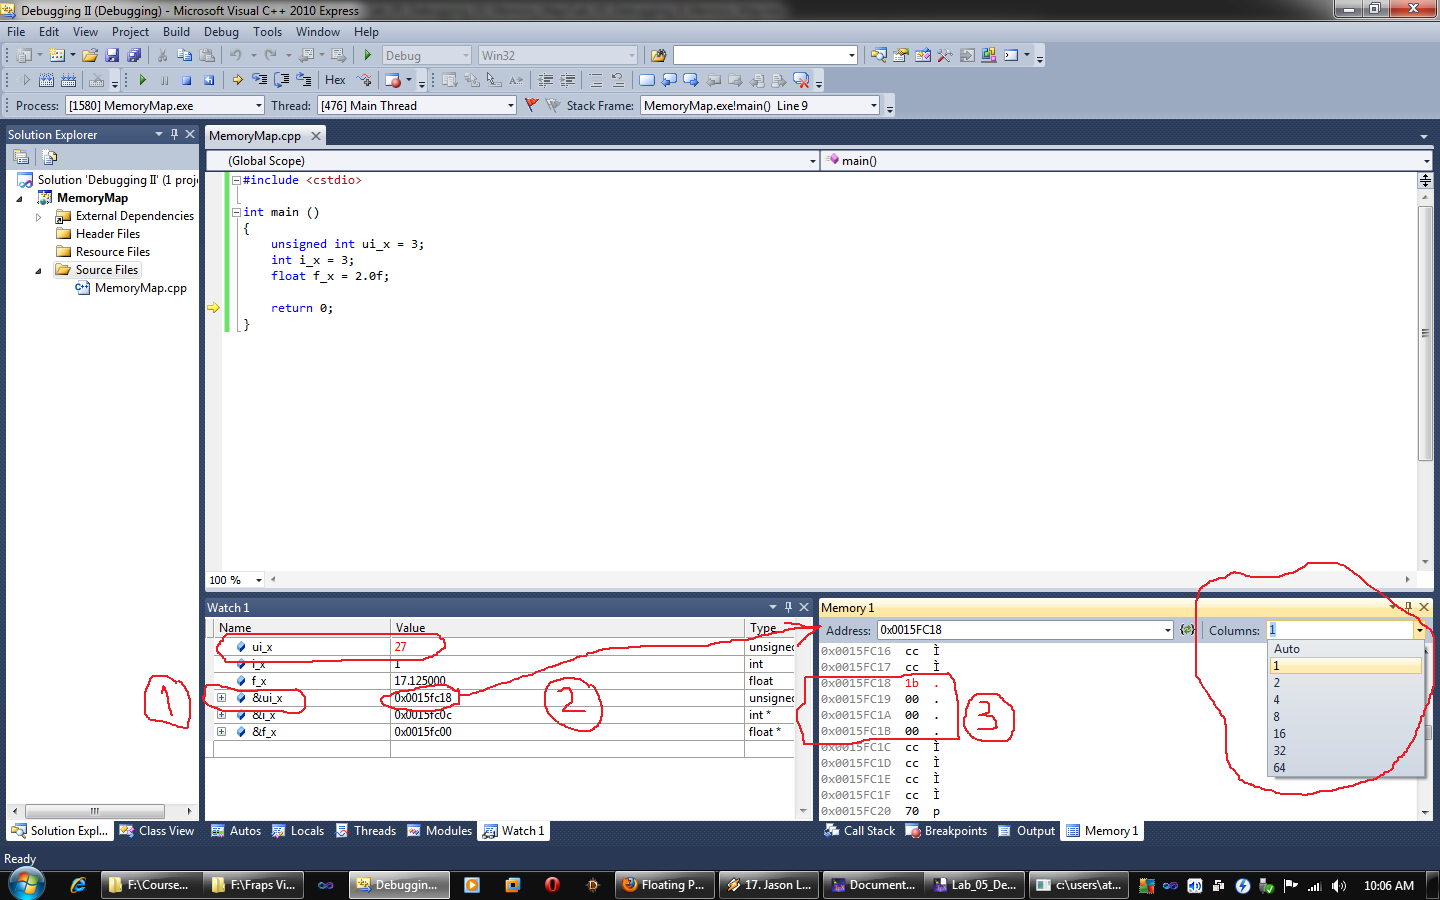
\includegraphics[width=0.95\textwidth]{DebuggerLayout.png}
\caption{Viewing value of a variable in memory}
\end{figure}

\begin{figure}[H]
\centering
\label{Adding-Memory-Window}
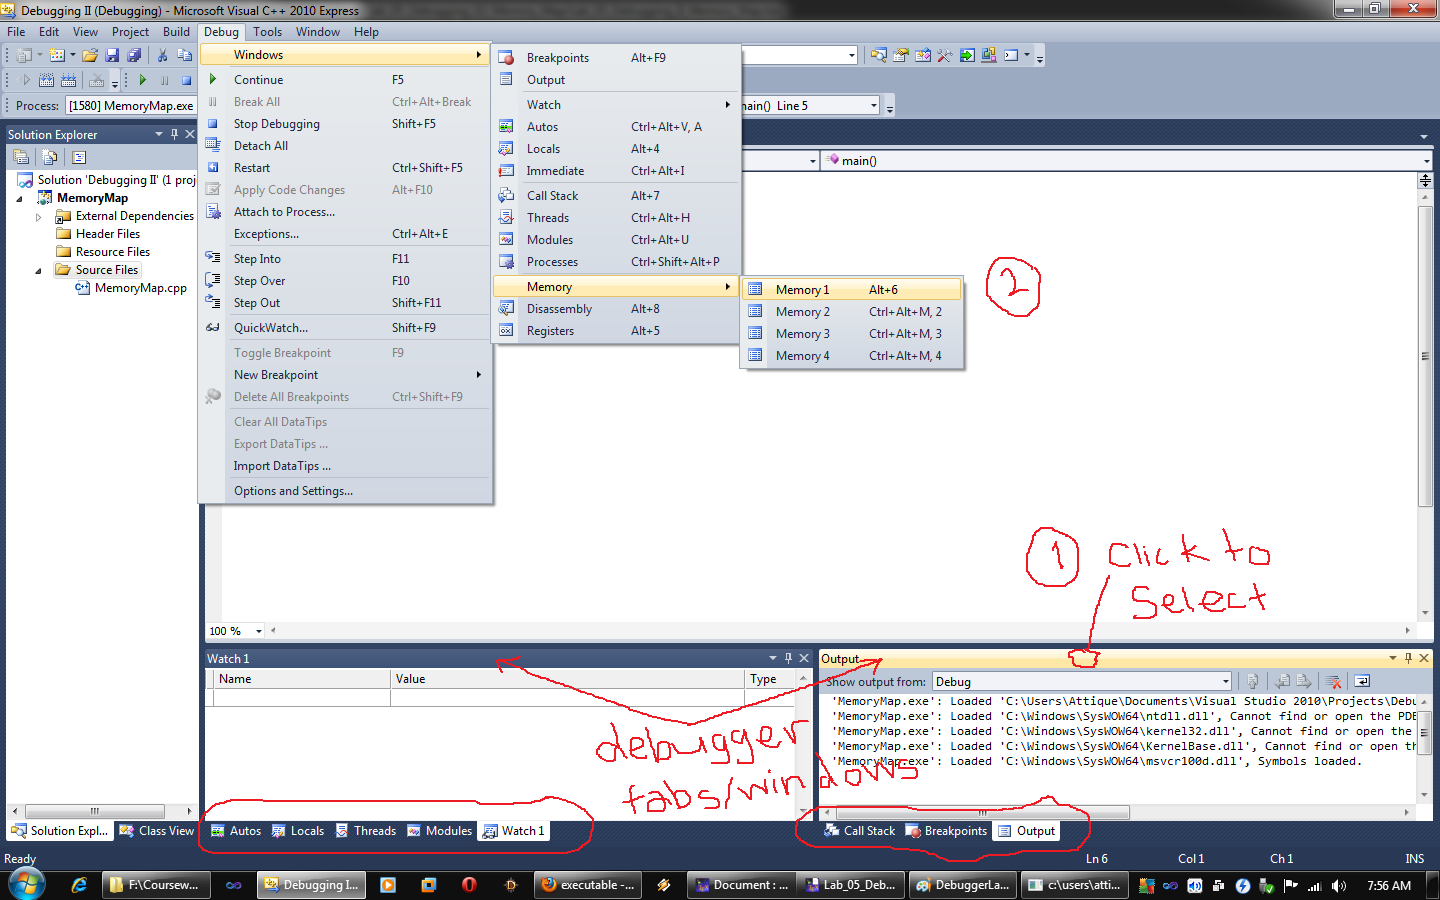
\includegraphics[width=0.95\textwidth]{AddingMemoryWindow.png}
\caption{Adding memory window}
\end{figure}
\section{Comparison Operators}
The comparison operators can be used to compare two values. The values can also be variables.  For example, \verb|x == y|. This should be read as \textit{Is x equal to y?} Most commonly used operators are:
\begin{itemize}
\item \verb|==| (equals?)
\item \verb|!=| (not equals?)
\item \verb|>| (greater than?)
\item \verb|<| (less than?)
\item \verb|>=| (equals or greater than?)
\item \verb|<=| (equals or less than?)
\end{itemize}

\section{Conditional Statements}
The syntax for conditional statement is,
\begin{lstlisting}
if (condition...)
{
    do this if condition is true...
}
else
{
    do this if condition is false...
}
\end{lstlisting}
If the condition is evaluated to be 0 then it is false. If condition is non--zero it is true.
Operators in previous section are useful for testing a certain condition. For example,
\begin{lstlisting}
int x = 2;
int y = 4;
if (x == y)
{
    cout << "x is equal to y" << endl;
}
else
{
   cout << "x is not equal to y" endl;
}
\end{lstlisting}
In this case the output will be \verb|x is not equal to y|. The \verb|else| part is not mandatory and an \verb|if| statement can be used standalone. For example,
\begin{lstlisting}
int x;
cin >> x;
if (x > 0)
{
    cout << "You have entered a positive number" << endl;
}
\end{lstlisting}
\section{Exercises/Lab Tasks}
\textbf{Note: You \emph{must} show all paperwork to get full marks}
\subsection{Task 1: Unsigned Integers}
Take the last three digits of your roll number. On paper how would this be stored as an unsigned integer in memory? Does your paperwork match the actual value shown in debugger?
\subsection{Task 2: Signed Integers}
Repeat the previous exercise assuming the number was negative.
\subsection{Task 3: Conditional Statements}
Make a program that takes in three numbers and determines the largest number.
\end{document}